\subsubsectionwithauthor[author={Mika Landeck},email={mika.landeck@fau.de}]{Aufgabe 5: Komplexitätstheorie}
\begin{teile}
 
	\item 
	Ein Minimalbeispiel für einen Graphen, der eine Beinahe-3-Färbung aber keine 3-Färbung besitzt, sieht wie folgt aus:

	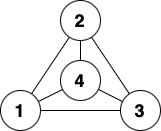
\includegraphics[scale=0.6]{minimal_graph_beinahe-drei-faerbung}
	
	Der Graph besitzt keine 3-Färbung, da Knoten $1,2,3$ und $4$ alle jeweils paarweise durch Kanten verbunden sind. Wenn also Knoten $1,2$ und $3$ mit drei verschiedenen Farben belegt werden, muss für $4$ ebenfalls eine dieser drei Farben gewählt werden und es entsteht eine Kante, die zwei Knoten mit gleicher Farbe verbindet. Folglich besitzt der Graph aber eine Beinahe-3-Färbung.

	\item
	Zunächst werden die genannten Entscheidungsprobleme in formale Sprachen übersetzt:

	$L_{B3F} = \{c(G)\ |\ G=(V,E) \text{ ist Graph, für den eine Beinahe-3-Färbung existiert}\}$

	$L_{3F} = \{c(G)\ |\ G=(V,E) \text{ ist Graph, für den eine 3-Färbung existiert}\}$

	Um zu zeigen, dass das Problem $B3F$ in $\mathcal{NP}$ liegt, wird eine NTM beschrieben, welche $L_{B3F}$ in polynomieller Zeit entscheidet:
	\begin{enumerate}
		\item Durchlaufe den Graphen Knoten für Knoten. ($O(n)$)
		\item Wähle jeweils nichtdeterministisch die passende Farbe, sodass am Ende möglichst wenige Kanten aus zwei gleichfarbigen Knoten entstehen. ($O(1)$)
		\item Gehe alle Kanten durch und überprüfe, ob höchstens eine Kante aus zwei gleichfarbigen Knoten gebildet wird. Wenn das der Fall ist akzeptiere, ansonsten halte und akzeptiere nicht. ($O(n)$)
	\end{enumerate}

	Nun wird eine polynomielle Komplexitäts-Reduktion von $B3F$ auf $3F$ durchgeführt. Dazu wird eine totale und in polynomieller Zeit berechenbare Funktion $f$ benötigt, die Probleme aus $3F$ auf Probleme aus $B3F$ abbildet:

	Sei $f:\Sigma^*\rightarrow \Sigma^*$ definiert über

	$f(w)= \begin{cases}
		c(V\cup \{v_1,v_2,v_3,v_4\}, E\ \cup \{(v_1,v_2),(v_1,v_3), &, falls\ w=c(V,E)\ mit\\
		(v_1,v_4),(v_2,v_3),(v_2,v_4),(v_3,v_4)\}) &\ G = (V,E)\ ist\ Graph\\
		0 &, sonst
	\end{cases}$
	
	$f$ ist offensichtlich total. Außerdem lässt sich eine DTM konstruieren, die $f$ in polynomieller Laufzeit berechnet:
	\begin{itemize}
		\item Syntaxcheck, ob $w=c(V,E)$ mit $e_1,e_2 \in E$ und $G = (V,E)$ ist Graph ($O(n)$).
		\item Passendes anhängen der entsprechenden Knoten und Kanten an Eingabe zu $c(V \cup \{v_1,v_2,v_3,v_4\}, E \cup \{(v_1,v_2),(v_1,v_3),(v_1,v_4),(v_2,v_3),(v_2,v_4),(v_3,v_4)\})$ ($O(n^2)$)
	\end{itemize}

	Es bleibt noch zu zeigen, dass $w \in L_{3F} \Leftrightarrow f(w) \in L_{B3F}$ gilt. Dies beweisen folgende Äquivalenzumformungen ($\forall w \in \Sigma^*$):
	\begin{align*}
		w \in L_{3F} \Longleftrightarrow\ & w=c(V,E)\ mit\ Graph\ G=(V,E)\ besitzt\ eine\ \text{3-Färbung}\\
		\Leftrightarrow\ & f(w)=c(V':=V \cup \{v_1,v_2,v_3,v_4\}, E':=E \cup \{(v_1,v_2),(v_1,v_3),(v_1,v_4),\\
		&\ (v_2,v_3),(v_2,v_4),(v_3,v_4)\})\ mit\ Graph\ G=(V,E)\ besitzt\ eine\ \text{3-Färbung}\\
		\Leftrightarrow\ & f(w)=c(V', E')\ mit\ Graph\ G'=(V',E')\ besitzt\ eine\ \text{Beinahe-3-Färbung}\\
		\Leftrightarrow\ & f(w) \in L_{B3F}
	\end{align*}
	\textit{Informelle Beschreibung: Minimalgraphen aus (a) zum Eingabegraphen hinzufügen. Somit wird eine 3-Färbung von $G$ zu einer Beinahe-3-Färbung von $G'$ und umgekehrt.}

	$B3F$ ist also $\mathcal{NP}$-hart und liegt in $\mathcal{NP}$. Somit ist $B3F$ $\mathcal{NP}$-vollständig.

\end{teile